\documentclass{beamer}

%
% Common preamble for all three parts.
%

%\usepackage[english]{babel}
\usepackage[polutonikogreek, italian]{babel}
\usepackage{amsmath}
\usepackage{color}
\usepackage[cache=false]{minted}
\usepackage{hyperref}
\usepackage{multicol}
\usepackage{tabularx}
\usepackage{tikz}
\usepackage{shapepar}

% only inline todonotes work
\usepackage{xkeyval}
\usepackage[textsize=small]{todonotes}
\presetkeys{todonotes}{inline}{}

\usetikzlibrary{shapes,arrows,positioning,shadows}

% no nav buttons
\usenavigationsymbolstemplate{}

\newcommand{\bftt}[1]{\textbf{\texttt{#1}}}
\newcommand{\comment}[1]{{\color[HTML]{008080}\textit{\textbf{\texttt{#1}}}}}
\newcommand{\cmd}[1]{{\color[HTML]{008000}\bftt{#1}}}
\newcommand{\bs}{\char`\\}
\newcommand{\cmdbs}[1]{\cmd{\bs#1}}
\newcommand{\lcb}{\char '173}
\newcommand{\rcb}{\char '175}
\newcommand{\cmdbegin}[1]{\cmdbs{begin\lcb}\bftt{#1}\cmd{\rcb}}
\newcommand{\cmdend}[1]{\cmdbs{end\lcb}\bftt{#1}\cmd{\rcb}}

\newcommand{\wllogo}{\textbf{Overleaf}}

% this is where the example source files are loaded from
% do not include a trailing slash
\newcommand{\fileuri}{https://raw.github.com/mirtexxan/latex-course/master/it}

\newcommand{\wlserver}{https://www.overleaf.com}
\newcommand{\wlnewdoc}[1]{\wlserver/docs?snip\_uri=\fileuri/#1\&splash=none}

\def\tikzname{Ti\emph{k}Z}

% from http://tex.stackexchange.com/questions/5226/keyboard-font-for-latex
\newcommand*\keystroke[1]{%
  \tikz[baseline=(key.base)]
    \node[%
      draw,
      fill=white,
      drop shadow={shadow xshift=0.25ex,shadow yshift=-0.25ex,fill=black,opacity=0.75},
      rectangle,
      rounded corners=2pt,
      inner sep=1pt,
      line width=0.5pt,
      font=\scriptsize\sffamily
    ](key) {#1\strut}
  ;
}
\newcommand{\keystrokebftt}[1]{\keystroke{\bftt{#1}}}

% stolen from minted.dtx
\newenvironment{exampletwoup}
  {\VerbatimEnvironment
   \begin{VerbatimOut}{example.out}}
  {\end{VerbatimOut}
   \setlength{\parindent}{0pt}
   \fbox{\begin{tabular}{l|l}
   \begin{minipage}{0.55\linewidth}
     \inputminted[fontsize=\small,resetmargins]{latex}{example.out}
   \end{minipage} &
   \begin{minipage}{0.35\linewidth}
     \input{example.out}
   \end{minipage}
   \end{tabular}}}

\newenvironment{exampletwouptiny}
  {\VerbatimEnvironment
   \begin{VerbatimOut}{example.out}}
  {\end{VerbatimOut}
   \setlength{\parindent}{0pt}
   \fbox{\begin{tabular}{l|l}
   \begin{minipage}{0.55\linewidth}
     \inputminted[fontsize=\scriptsize,resetmargins]{latex}{example.out}
   \end{minipage} &
   \begin{minipage}{0.35\linewidth}
     \setlength{\parskip}{6pt plus 1pt minus 1pt}%
     \raggedright\scriptsize\input{example.out}
   \end{minipage}
   \end{tabular}}}

\newenvironment{exampletwouptinynoframe}
  {\VerbatimEnvironment
   \begin{VerbatimOut}{example.out}}
  {\end{VerbatimOut}
   \setlength{\parindent}{0pt}
   \begin{tabular}{l|l}
   \begin{minipage}{0.55\linewidth}
     \inputminted[fontsize=\scriptsize,resetmargins]{latex}{example.out}
   \end{minipage} &
   \begin{minipage}{0.35\linewidth}
     \setlength{\parskip}{6pt plus 1pt minus 1pt}%
     \raggedright\scriptsize\input{example.out}
   \end{minipage}
   \end{tabular}}

\title{Muovere i primi passi con \LaTeX}
\author{Mirto Musci, PhD}
\institute{Assegnista di ricerca, Universit\`a di Pavia\\
Dipartimento di Ingegneria Industriale e dell'Informazione}
\titlegraphic{%
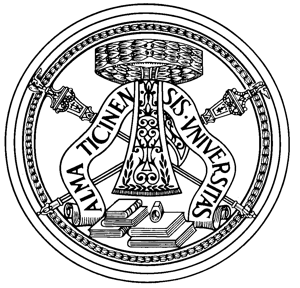
\includegraphics[height=1.8cm]{Unipv-logo}\hspace{1cm}

\includegraphics[height=1.8cm]{nuovo}%\hspace{1.2cm}
%
\includegraphics[height=36pt]{overleaf}\\[1em]
}


\subtitle{Parte 4: Scrivere una tesi di laurea con Latex}

\begin{document}

%%%%%%%%%%%%%%%%%%%%%%%%%%%%%%%%%%%%%%%%%%%%%%%%%%%%%%%%%%%%%%%%%%%%%%%%%%%%%%%
%%%%%%%%%%%%%%%%%%%%%%%%%%%%%%%%%%%%%%%%%%%%%%%%%%%%%%%%%%%%%%%%%%%%%%%%%%%%%%%
%%%%%%%%%%%%%%%%%%%%%%%%%%%%%%%%%%%%%%%%%%%%%%%%%%%%%%%%%%%%%%%%%%%%%%%%%%%%%%%
\begin{frame}
\titlepage
\end{frame}

%%%%%%%%%%%%%%%%%%%%%%%%%%%%%%%%%%%%%%%%%%%%%%%%%%%%%%%%%%%%%%%%%%%%%%%%%%%%%%%
%%%%%%%%%%%%%%%%%%%%%%%%%%%%%%%%%%%%%%%%%%%%%%%%%%%%%%%%%%%%%%%%%%%%%%%%%%%%%%%
%%%%%%%%%%%%%%%%%%%%%%%%%%%%%%%%%%%%%%%%%%%%%%%%%%%%%%%%%%%%%%%%%%%%%%%%%%%%%%%
\begin{frame}{Struttura di base}
\begin{itemize}
\item Dichiarazione della \structure{classe} (\cmd{book} o \cmd{amsbook})
\item Preambolo (cosa includere?)
\item \cmdbegin{document}
\item Documento
\begin{itemize}
\item Materiale \structure{iniziale}
\item Materiale \structure{principale}
\item Materiale \structure{finale}
\end{itemize}
\item \cmdend{document}
\end{itemize}
\end{frame}

%%%%%%%%%%%%%%%%%%%%%%%%%%%%%%%%%%%%%%%%%%%%%%%%%%%%%%%%%%%%%%%%%%%%%%%%%%%%%%%
%%%%%%%%%%%%%%%%%%%%%%%%%%%%%%%%%%%%%%%%%%%%%%%%%%%%%%%%%%%%%%%%%%%%%%%%%%%%%%%
%%%%%%%%%%%%%%%%%%%%%%%%%%%%%%%%%%%%%%%%%%%%%%%%%%%%%%%%%%%%%%%%%%%%%%%%%%%%%%%
\begin{frame}{Materiale preliminare}

\begin{block}{Il materiale preliminare di una tesi \textit{deve} contenere}
\begin{itemize}
\item Un frontespizio, con il titolo e le informazioni necessarie
\item Un indice
\end{itemize}
\end{block}

\begin{block}{Il materiale preliminare di una tesi \textit{pu\`o} contenere}
\begin{itemize}
\item Una dedica
\item Una lista delle figure
\item Una lista delle tabelle
\item Altre liste di oggetti particolari (es. algoritmi)
\item Una prefazione
\item Un'introduzione
\end{itemize}
\end{block}

\end{frame}

%%%%%%%%%%%%%%%%%%%%%%%%%%%%%%%%%%%%%%%%%%%%%%%%%%%%%%%%%%%%%%%%%%%%%%%%%%%%%%%
%%%%%%%%%%%%%%%%%%%%%%%%%%%%%%%%%%%%%%%%%%%%%%%%%%%%%%%%%%%%%%%%%%%%%%%%%%%%%%%
%%%%%%%%%%%%%%%%%%%%%%%%%%%%%%%%%%%%%%%%%%%%%%%%%%%%%%%%%%%%%%%%%%%%%%%%%%%%%%%
\begin{frame}{Materiale principale e finale}

\begin{block}{Il materiale principale di una tesi \textit{deve} contenere}
\begin{itemize}
\item Un'introduzione
\item I \textit{capitoli} in cui la tesi viene sviluppata
\item Una bibliografia
\end{itemize}
\end{block}

\begin{block}{Il materiale principale di una tesi \textit{pu\`o} contenere}
\begin{itemize}
\item Una o pi\`u appendici
\end{itemize}
\end{block}

\begin{block}{Il materiale finale di una tesi \textit{pu\`o} contenere}
\begin{itemize}
\item Una o pi\`u appendici
\item Un glossario dei principali termini usati
\item Un indice analitico
\end{itemize}
\end{block}

\end{frame}

%%%%%%%%%%%%%%%%%%%%%%%%%%%%%%%%%%%%%%%%%%%%%%%%%%%%%%%%%%%%%%%%%%%%%%%%%%%%%%%
%%%%%%%%%%%%%%%%%%%%%%%%%%%%%%%%%%%%%%%%%%%%%%%%%%%%%%%%%%%%%%%%%%%%%%%%%%%%%%%
%%%%%%%%%%%%%%%%%%%%%%%%%%%%%%%%%%%%%%%%%%%%%%%%%%%%%%%%%%%%%%%%%%%%%%%%%%%%%%%
\begin{frame}{Apparenti contraddizioni?}
\begin{itemize}
\item L'introduzione appartiene al materiale preliminare o principale?
\item Le appendici appartengono al materiale principale o finale?
\item La risposta \`e: \alert{dipende}
\end{itemize}
\bigskip
\small
L'introduzione fa parte, normalmente, del materiale principale. In tal caso deve essere un
capitolo numerato come gli altri. Se \`e breve e non contiene che una sintetica esposizione del problema, pu\`o andare nel materiale preliminare e non sar\`a numerata.

\bigskip
Se le appendici consistono solo del codice dei programmi usati nello sviluppo,
probabilmente vanno nel materiale finale. Se l'appendice però consiste del codice per un
programma che applica in modo originale le idee sviluppate, sar\`a parte del materiale
principale. Il problema \`e tutto sommato poco importante. Va risolto caso per caso.\end{frame}

%%%%%%%%%%%%%%%%%%%%%%%%%%%%%%%%%%%%%%%%%%%%%%%%%%%%%%%%%%%%%%%%%%%%%%%%%%%%%%%
%%%%%%%%%%%%%%%%%%%%%%%%%%%%%%%%%%%%%%%%%%%%%%%%%%%%%%%%%%%%%%%%%%%%%%%%%%%%%%%
%%%%%%%%%%%%%%%%%%%%%%%%%%%%%%%%%%%%%%%%%%%%%%%%%%%%%%%%%%%%%%%%%%%%%%%%%%%%%%%
\begin{frame}[fragile]{Preambolo: margini}

\begin{itemize}
\item Di base \LaTeX{} ha margini molto larghi. Per modificare le impostazione predefinite, si usa il pacchetto \cmd{geometry}:

\begin{minted}[frame=single]{latex}
\usepackage[top=2.8cm, bottom=2.5cm,
	left=2.1cm, right=1.7cm]{geometry}
\end{minted}
\item Una volta scelti i parametri serve specificare se il documento sar\`a \structure{fronte-retro} (FR) o \structure{solo-fronte} (SF)
\item Nel caso SF \`e sufficiente l'opzione \cmd{oneside}. Nel caso FR serve invece l'opzione \cmd{twoside}
\begin{minted}[frame=single]{latex}
\documentclass[...,oneside,...]{book|article}
\documentclass[...,twoside,...]{book|article}
\end{minted}
\item Se lo si vuole FR ma con i margini fissi, allora si usa sempre la stessa opzione, ma si altera il comando geometry:
\begin{minted}[frame=single]{latex}
\usepackage[asymmetric,...]{geometry}
\end{minted}
\end{itemize}

\end{frame}

%%%%%%%%%%%%%%%%%%%%%%%%%%%%%%%%%%%%%%%%%%%%%%%%%%%%%%%%%%%%%%%%%%%%%%%%%%%%%%%
%%%%%%%%%%%%%%%%%%%%%%%%%%%%%%%%%%%%%%%%%%%%%%%%%%%%%%%%%%%%%%%%%%%%%%%%%%%%%%%
%%%%%%%%%%%%%%%%%%%%%%%%%%%%%%%%%%%%%%%%%%%%%%%%%%%%%%%%%%%%%%%%%%%%%%%%%%%%%%%
\begin{frame}[fragile]{Preambolo: miscellanea}
\begin{itemize}
\item Per modificare l'interlinea si usa il comando:
\begin{minted}[frame=single]{latex}
\linespread{1.5}
\end{minted}
\item Per iniziare un paragrafo con una lettera miniata si usa il pacchetto \cmd{lettrine}
\begin{exampletwouptiny}
\lettrine{E}{cco} un esempio.
\end{exampletwouptiny}
\item Attraverso il pacchetto \cmd{bookmark} \`e possibile rendere il proprio file pi\`u facile alla lettura. Le impostazioni:

\begin{minted}[frame=single]{latex}
\usepackage[open, openlevel=1]{bookmark}
\end{minted}
rendono il file \structure{navigabile}, ovvero ogni elemento dell'indice e della bibliografia diventano dei collegamenti ipertestuali.
\end{itemize}

\end{frame}

%%%%%%%%%%%%%%%%%%%%%%%%%%%%%%%%%%%%%%%%%%%%%%%%%%%%%%%%%%%%%%%%%%%%%%%%%%%%%%%
%%%%%%%%%%%%%%%%%%%%%%%%%%%%%%%%%%%%%%%%%%%%%%%%%%%%%%%%%%%%%%%%%%%%%%%%%%%%%%%
%%%%%%%%%%%%%%%%%%%%%%%%%%%%%%%%%%%%%%%%%%%%%%%%%%%%%%%%%%%%%%%%%%%%%%%%%%%%%%%
\begin{frame}[fragile]{Materiale preliminare}

\begin{itemize}
\item Tralasciamo per il momento il frontespizio\ldots
\item Se usiamo la classe \structure{book} o \structure{amsbook}, il primo comando dopo aver prodotto il frontespizio \`e:
\begin{center}
\Large\cmdbs{frontmatter}
\end{center}
\item La prima cosa da trattare \`e l'indice: una tesi deve averlo all'inizio, in modo che il lettore possa rapidamente trovare quello che cerca.
\item Come si produce l'indice?
\begin{center}
\Large\cmdbs{tableofcontents}
\end{center}
\item Per decidere cosa mettere nell'indice si usa:
\begin{minted}[frame=none]{latex}
\setcounter{tocdepth}{2}
\end{minted}
\item Il numero si riferisce ai comandi di sezionamento\\(es. \cmd{0} fino a chapter, \cmd{1} fino a section, \cmd{2} fino a subsection\ldots)

\end{itemize}


\end{frame}

%%%%%%%%%%%%%%%%%%%%%%%%%%%%%%%%%%%%%%%%%%%%%%%%%%%%%%%%%%%%%%%%%%%%%%%%%%%%%%%
%%%%%%%%%%%%%%%%%%%%%%%%%%%%%%%%%%%%%%%%%%%%%%%%%%%%%%%%%%%%%%%%%%%%%%%%%%%%%%%
%%%%%%%%%%%%%%%%%%%%%%%%%%%%%%%%%%%%%%%%%%%%%%%%%%%%%%%%%%%%%%%%%%%%%%%%%%%%%%%
\begin{frame}{Materiale preliminare}

Dopo l'indice, se necessario, potranno esserci:
\begin{itemize}
\item l'elenco delle figure $\rightarrow$ \cmdbs{listoffigures}
\item l'elenco delle tabelle$\rightarrow$ \cmdbs{listoftables}
\item una prefazione o l'introduzione; solitamente sono capitoli non numerati con sezioni non numerate:
\begin{center}
\Large\cmdbs{chapter*} \cmdbs{section*}
\end{center}
\item Per passare al materiale principale si usa
\begin{center}
\Large\cmdbs{mainmatter}
\end{center}
\item Similmente, per passare al materiale finale si usa:
\begin{center}
\Large\cmdbs{backmatter}
\end{center}
\end{itemize}
\end{frame}

%%%%%%%%%%%%%%%%%%%%%%%%%%%%%%%%%%%%%%%%%%%%%%%%%%%%%%%%%%%%%%%%%%%%%%%%%%%%%%%
%%%%%%%%%%%%%%%%%%%%%%%%%%%%%%%%%%%%%%%%%%%%%%%%%%%%%%%%%%%%%%%%%%%%%%%%%%%%%%%
%%%%%%%%%%%%%%%%%%%%%%%%%%%%%%%%%%%%%%%%%%%%%%%%%%%%%%%%%%%%%%%%%%%%%%%%%%%%%%%
\begin{frame}{Materiale principale: inserire sorgenti in \LaTeX{}}

\begin{itemize}
\item Per riportare parti di codice \`e possibile usare il pacchetto \cmd{listing}
tramite l'ambiente \cmd{lstlisting}
\end{itemize}

\begin{minipage}{0.50\linewidth}
\inputminted[fontsize=\scriptsize,frame=single,resetmargins]{latex}%
  {listings.tex}
\end{minipage}
\begin{minipage}{0.45\linewidth}
% trim: l b r t
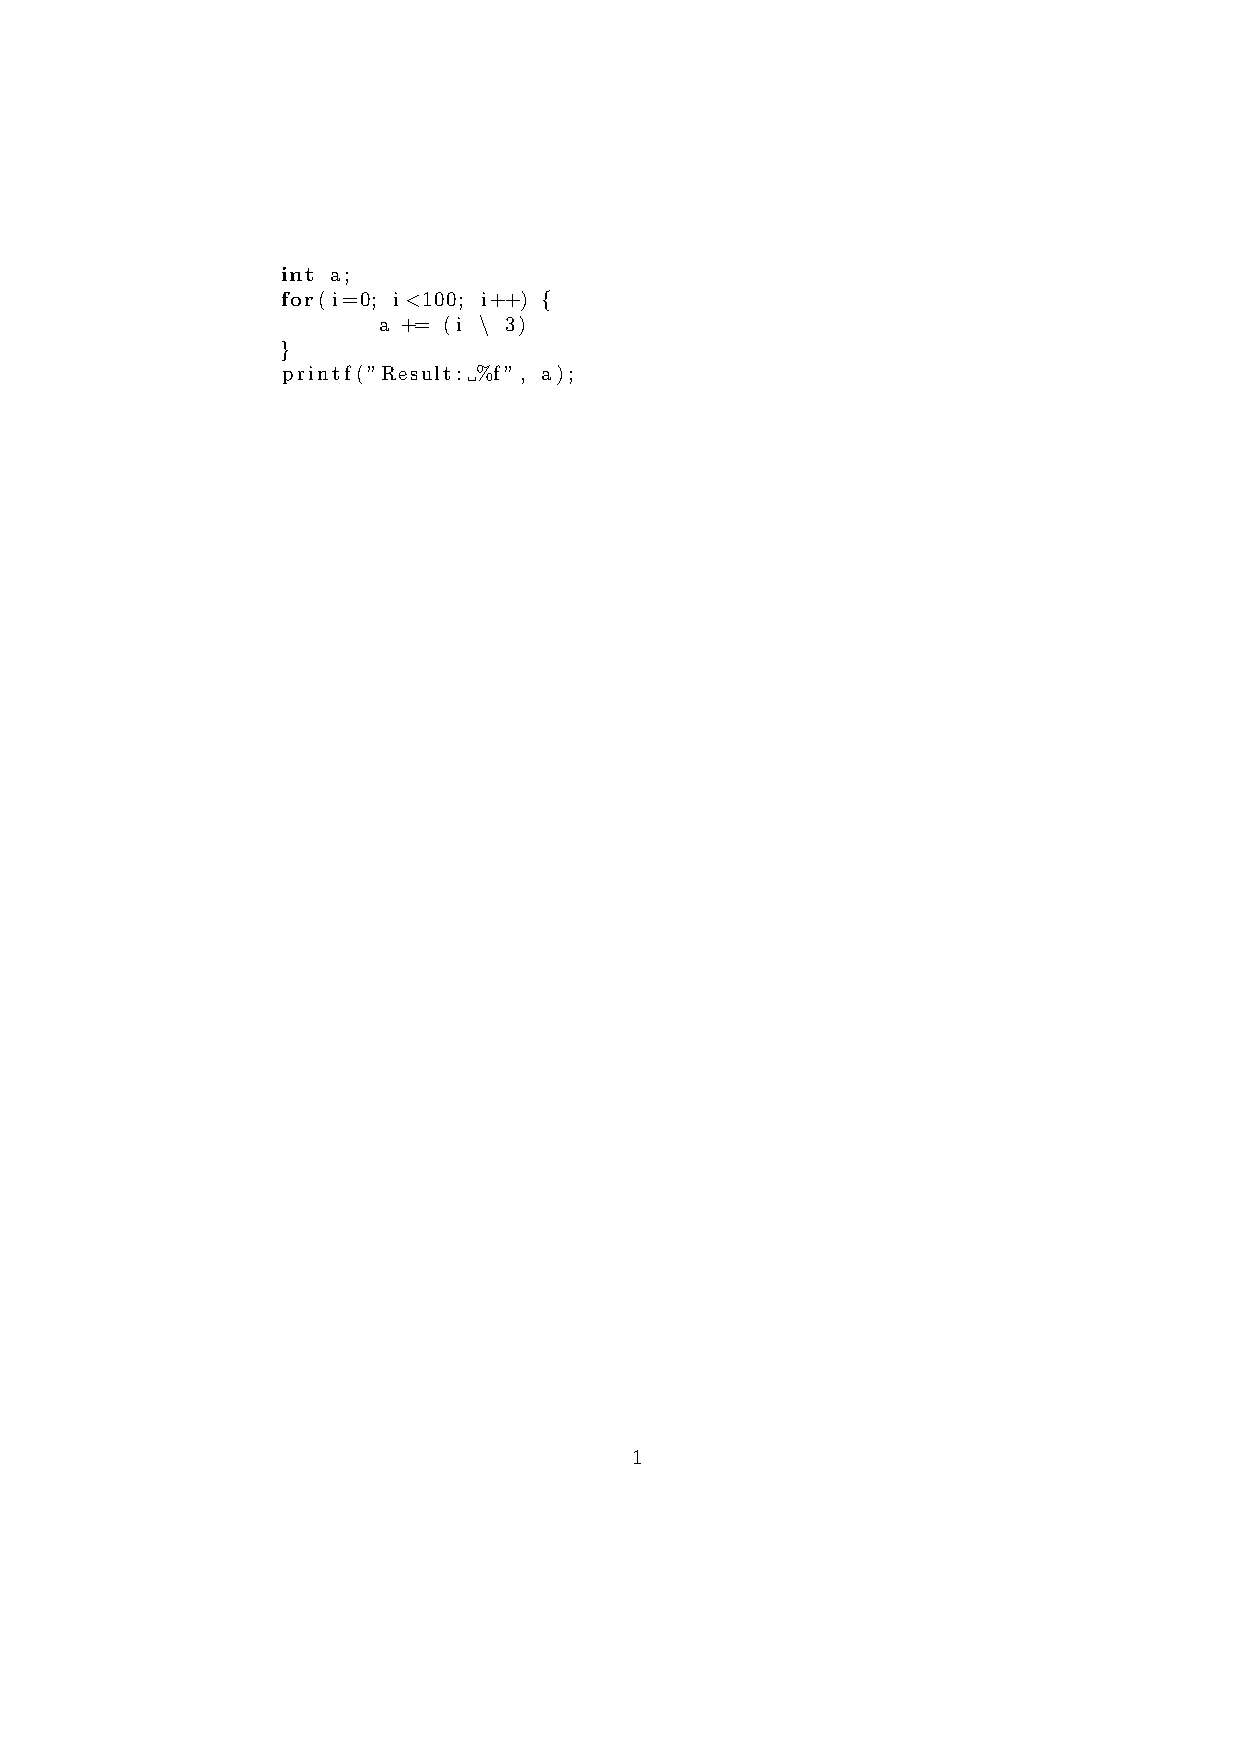
\includegraphics[width=\textwidth,clip,trim=1.5in 7in 4in 1in]{listings.pdf}
\end{minipage}

\end{frame}

%%%%%%%%%%%%%%%%%%%%%%%%%%%%%%%%%%%%%%%%%%%%%%%%%%%%%%%%%%%%%%%%%%%%%%%%%%%%%%%
%%%%%%%%%%%%%%%%%%%%%%%%%%%%%%%%%%%%%%%%%%%%%%%%%%%%%%%%%%%%%%%%%%%%%%%%%%%%%%%
%%%%%%%%%%%%%%%%%%%%%%%%%%%%%%%%%%%%%%%%%%%%%%%%%%%%%%%%%%%%%%%%%%%%%%%%%%%%%%%
\begin{frame}{Materiale principale: inserire strutture chimiche in \LaTeX{}}

\begin{itemize}
\item Per inserire strutture chimiche \`e sufficiente includere il pacchetto \cmd{chemfig}
\end{itemize}

\begin{minipage}{0.65\linewidth}
\inputminted[fontsize=\scriptsize,frame=single,resetmargins]{latex}%
  {chemfig_example.tex}
\end{minipage}
\begin{minipage}{0.30\linewidth}
% trim: l b r t
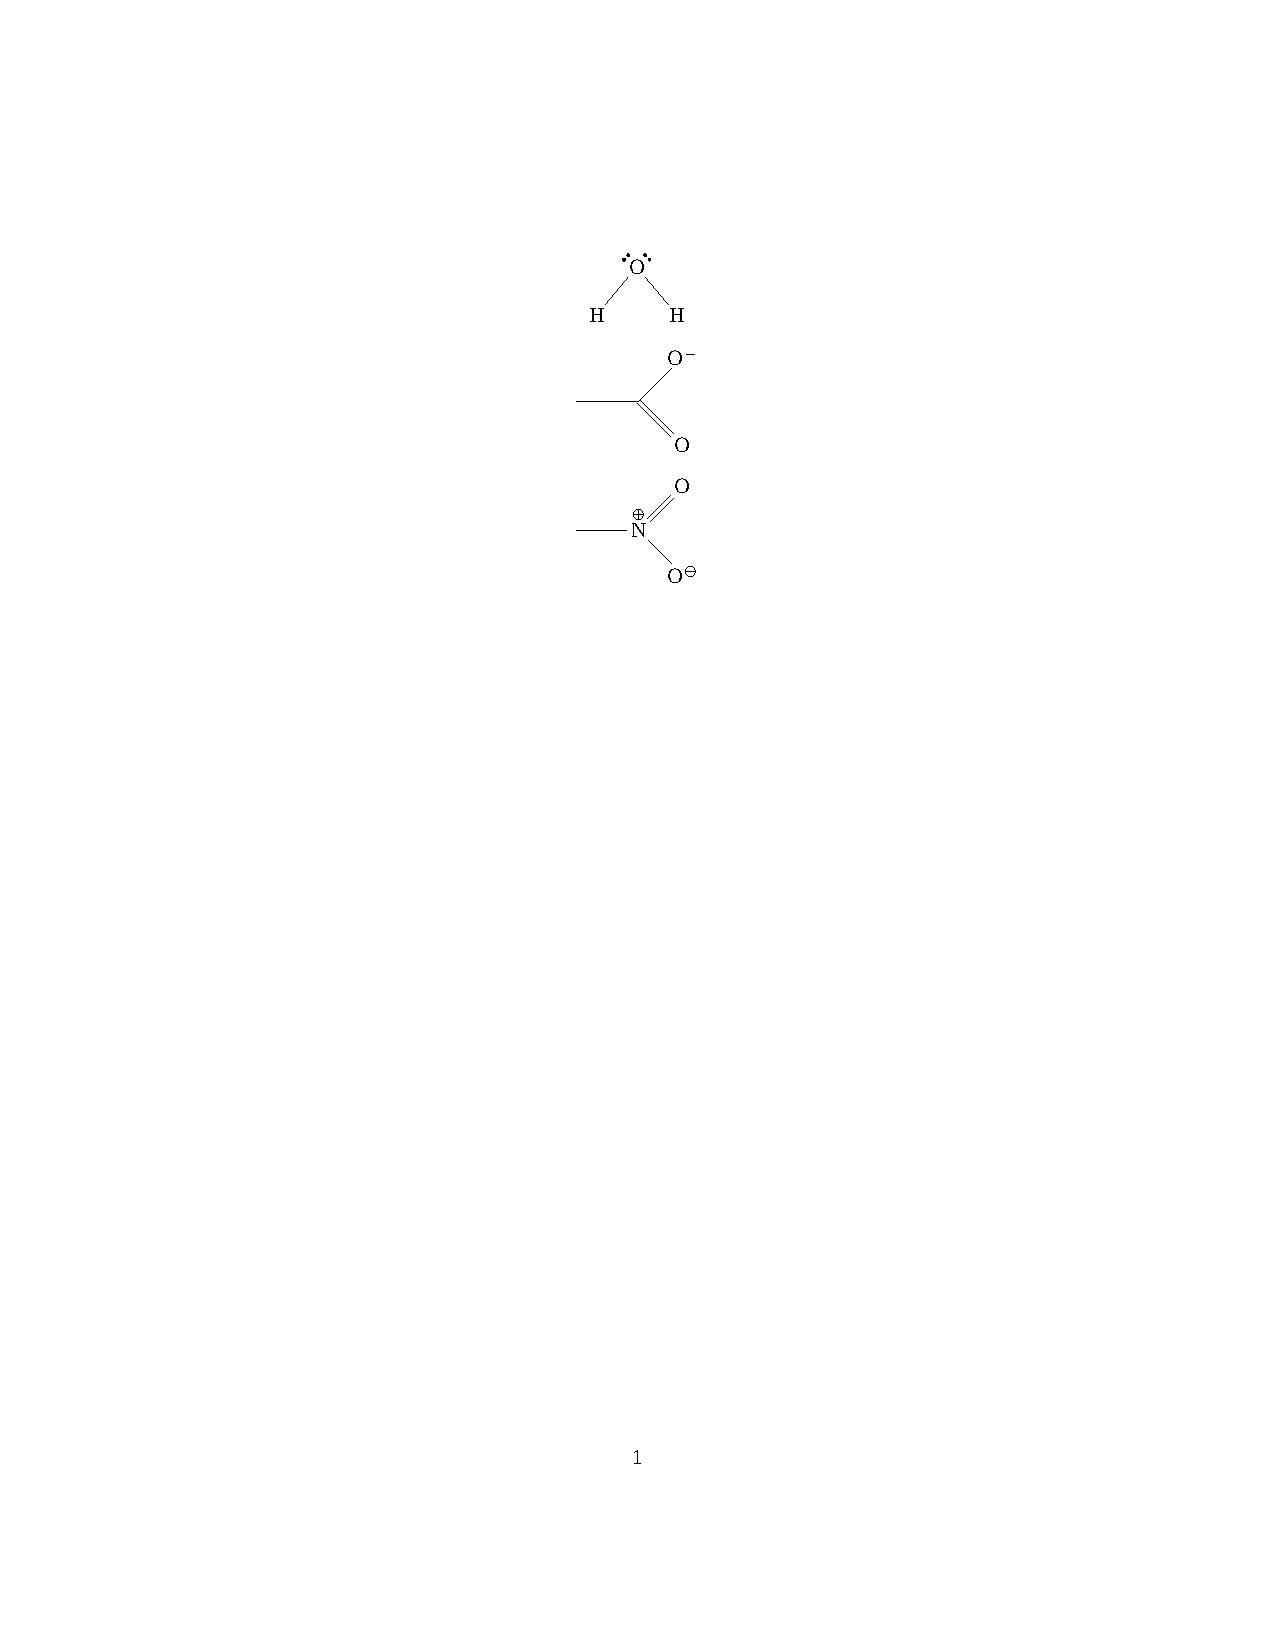
\includegraphics[width=\textwidth,clip,trim=3.5in 7in 3.5in 1.5in]{chemfig_example.pdf}
\end{minipage}

\end{frame}

%%%%%%%%%%%%%%%%%%%%%%%%%%%%%%%%%%%%%%%%%%%%%%%%%%%%%%%%%%%%%%%%%%%%%%%%%%%%%%%
%%%%%%%%%%%%%%%%%%%%%%%%%%%%%%%%%%%%%%%%%%%%%%%%%%%%%%%%%%%%%%%%%%%%%%%%%%%%%%%
%%%%%%%%%%%%%%%%%%%%%%%%%%%%%%%%%%%%%%%%%%%%%%%%%%%%%%%%%%%%%%%%%%%%%%%%%%%%%%%
\begin{frame}{Numerazione delle pagine}
\begin{itemize}
\item Esistono diversi modi di \structure{numerare} le pagine
\begin{itemize}
\item roman (i, ii, iii, iv, \ldots)
\item arabic (1, 2, 3, 4, \ldots
\item Roman (I, II, III, IV, \ldots)
\item alph (a, b, c, e, j, \ldots)
\item Alph (A, B, C, E, J, \ldots)
\end{itemize}
\item \`E possibile impostare lo stesso stile di numerazione per tutto il testo o sceglierne diversi in base alla struttura con il comando:
\begin{center}
\Large\cmdbs{pagenumbering}
\end{center}
\item \cmdbs{frontmatter} usa la numerazione romana, \cmdbs{mainmatter} resetta la numerazione e usa quella araba, \cmdbs{backmatter} non tocca la numerazione
\end{itemize}
\end{frame}

%%%%%%%%%%%%%%%%%%%%%%%%%%%%%%%%%%%%%%%%%%%%%%%%%%%%%%%%%%%%%%%%%%%%%%%%%%%%%%%
%%%%%%%%%%%%%%%%%%%%%%%%%%%%%%%%%%%%%%%%%%%%%%%%%%%%%%%%%%%%%%%%%%%%%%%%%%%%%%%
%%%%%%%%%%%%%%%%%%%%%%%%%%%%%%%%%%%%%%%%%%%%%%%%%%%%%%%%%%%%%%%%%%%%%%%%%%%%%%%
\begin{frame}[fragile]{Stili della testata e del pi\`e di pagina}

\begin{itemize}
\item Si usano i pacchetti \cmd{fancyhdr} e \cmd{lastpage}
\item \`E sufficiente inserire nel preambolo \mintinline{latex}!\pagestyle{stile}!
\item Le possibili opzioni:
\begin{itemize}
\item \emph{empty} (pagina vuota, solo testo)
\item \emph{plain} (pagina con numerazione centrata in basso)
\item \emph{headings }(in alto numero di pagina e capitolo)
\item \emph{fancy} per totale personalizzazione \ldots
\end{itemize}
\item Per documenti fronteretro andrebbero diversificati header e footer di pagine pari e pagine dispari\ldots
\end{itemize}
\end{frame}

%%%%%%%%%%%%%%%%%%%%%%%%%%%%%%%%%%%%%%%%%%%%%%%%%%%%%%%%%%%%%%%%%%%%%%%%%%%%%%%
%%%%%%%%%%%%%%%%%%%%%%%%%%%%%%%%%%%%%%%%%%%%%%%%%%%%%%%%%%%%%%%%%%%%%%%%%%%%%%%
%%%%%%%%%%%%%%%%%%%%%%%%%%%%%%%%%%%%%%%%%%%%%%%%%%%%%%%%%%%%%%%%%%%%%%%%%%%%%%%
\begin{frame}{Esempio stili}
\begin{minipage}{0.50\linewidth}
\inputminted[fontsize=\scriptsize,frame=single,resetmargins]{latex}%
  {style.tex}
\end{minipage}
\begin{minipage}{0.45\linewidth}
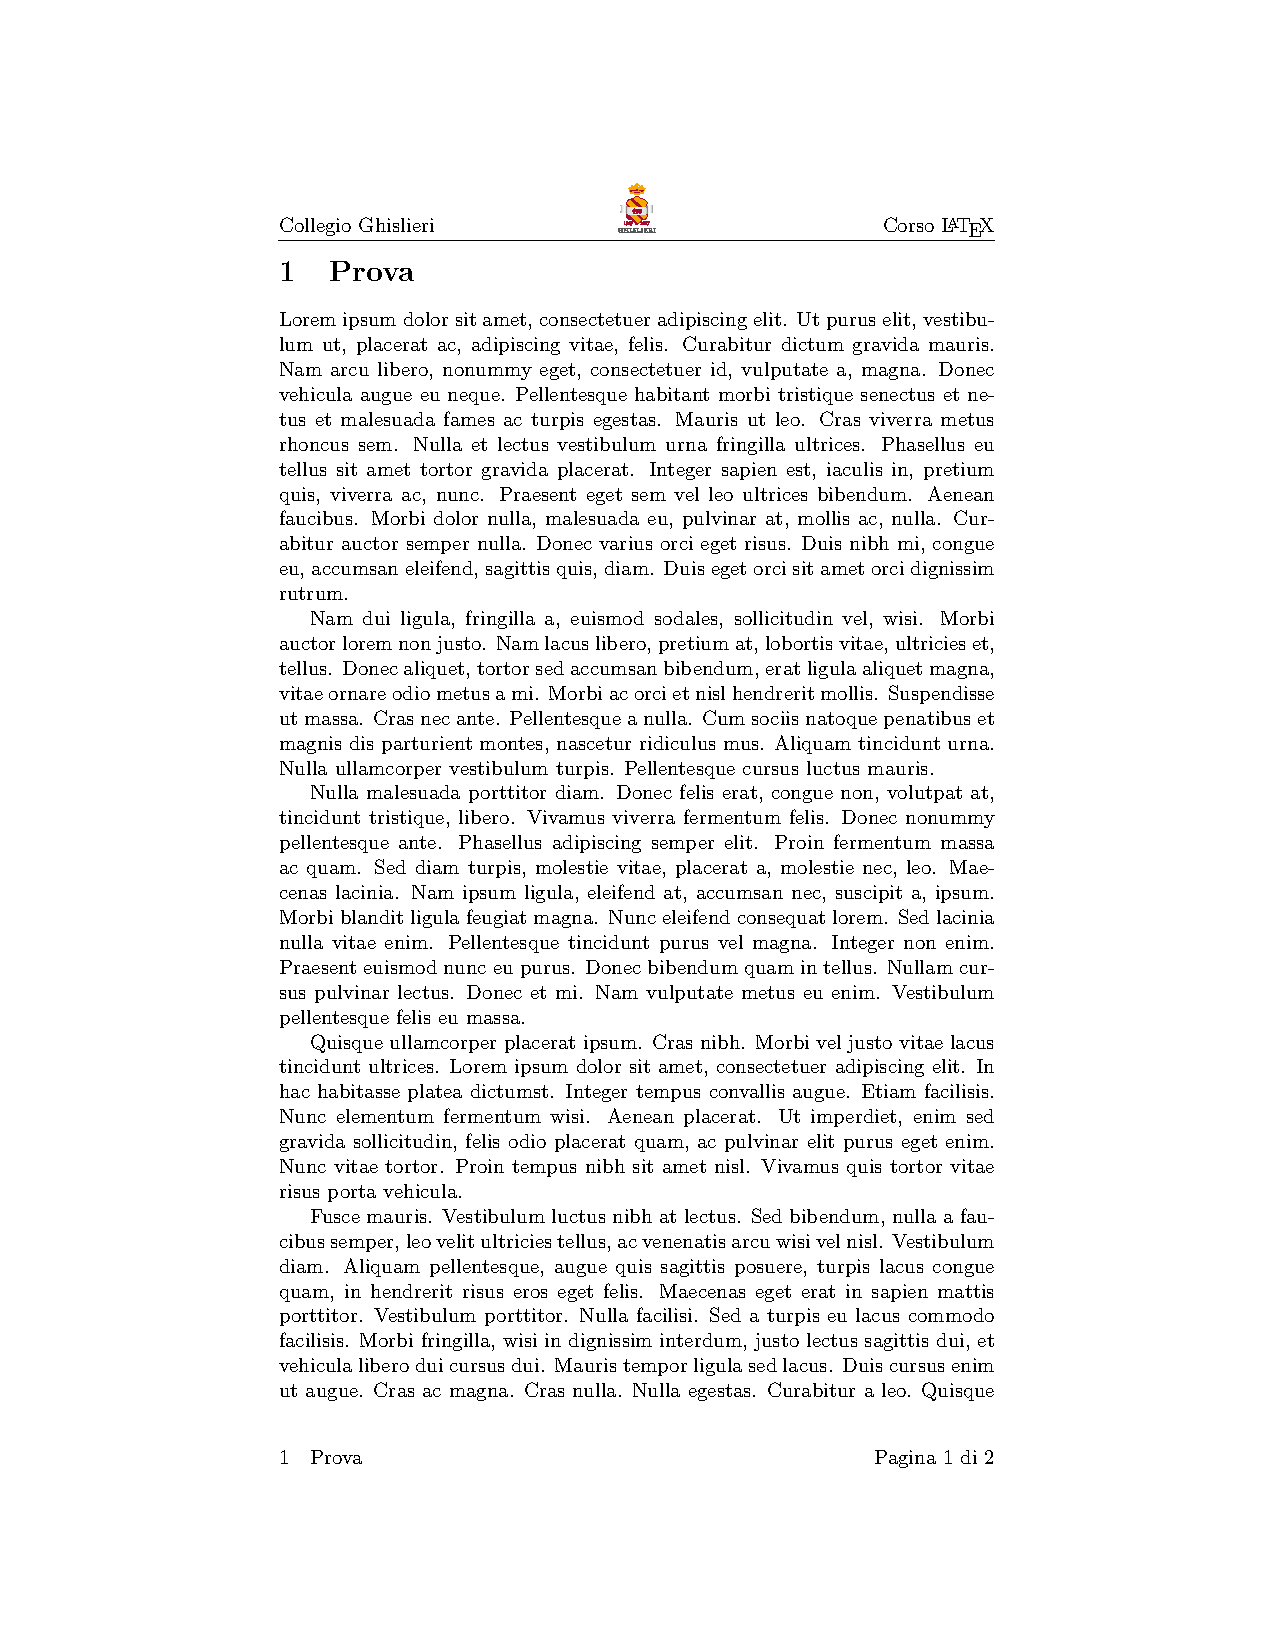
\includegraphics[width=\textwidth,clip,trim=1.5in 0.5in 1.5in 1in]{style.pdf}
\end{minipage}
\end{frame}

%%%%%%%%%%%%%%%%%%%%%%%%%%%%%%%%%%%%%%%%%%%%%%%%%%%%%%%%%%%%%%%%%%%%%%%%%%%%%%%
%%%%%%%%%%%%%%%%%%%%%%%%%%%%%%%%%%%%%%%%%%%%%%%%%%%%%%%%%%%%%%%%%%%%%%%%%%%%%%%
%%%%%%%%%%%%%%%%%%%%%%%%%%%%%%%%%%%%%%%%%%%%%%%%%%%%%%%%%%%%%%%%%%%%%%%%%%%%%%%
\begin{frame}{Esercizio: scheletro di una tesi}

\inputminted[fontsize=\scriptsize,frame=single,resetmargins]{latex}%
  {thesis.tex}

\end{frame}

%%%%%%%%%%%%%%%%%%%%%%%%%%%%%%%%%%%%%%%%%%%%%%%%%%%%%%%%%%%%%%%%%%%%%%%%%%%%%%%
%%%%%%%%%%%%%%%%%%%%%%%%%%%%%%%%%%%%%%%%%%%%%%%%%%%%%%%%%%%%%%%%%%%%%%%%%%%%%%%
%%%%%%%%%%%%%%%%%%%%%%%%%%%%%%%%%%%%%%%%%%%%%%%%%%%%%%%%%%%%%%%%%%%%%%%%%%%%%%%
\begin{frame}{Esercizio: adesso tocca a voi!}
\begin{itemize}
\item Provate ad abbozzare la \structure{vostra} tesi di laurea.
\item Niente pi\`u aiuti: dovete partire da zero!
\end{itemize}

\begin{block}{Obiettivi}
\begin{itemize}
\item Costruite il preambolo (classe, pacchetti aggiuntivi, etc.)
\item Indicate  materiale preliminare, principale e finale
\item Generate la pagina del titolo
\item Generate l'indice con il livello prescelto
\item Scrivete un abbozzo di introduzione e capitolo (consiglio: usate il pacchetto \cmd{lipsum} per generare testo.
\item Provate ad inserire riferimenti incrociati, bibliografia, elenchi, tabelle, figure, formule, sorgenti, ispirandovi liberamente agli esercizi delle lezioni passate\ldots
\end{itemize}
\end{block}

\end{frame}

%%%%%%%%%%%%%%%%%%%%%%%%%%%%%%%%%%%%%%%%%%%%%%%%%%%%%%%%%%%%%%%%%%%%%%%%%%%%%%%
%%%%%%%%%%%%%%%%%%%%%%%%%%%%%%%%%%%%%%%%%%%%%%%%%%%%%%%%%%%%%%%%%%%%%%%%%%%%%%%
%%%%%%%%%%%%%%%%%%%%%%%%%%%%%%%%%%%%%%%%%%%%%%%%%%%%%%%%%%%%%%%%%%%%%%%%%%%%%%%
\begin{frame}{Fine del corso}
\begin{center}
Ora siete pronte a lanciarvi nel mondo di \LaTeX{}!

In bocca al lupo!
\end{center}
\end{frame}

\end{document}
